\subsection{receiving a MacPkt}

On reception of a MacPkt from the MAC layer, \h{\bp} checks if:
\begin{enumerate}
	\item the radio is in TX state\req{sendPreqMode},
	\item it is not already sending a packet\req{sendPreqSending} and
	%\item the channel is idle\req{sendPreqIdle} (this is no hard
requirement, \h{\bp} could send anyway).
\end{enumerate} 

If one of these conditions is not fulfilled it will throw an error.\\

The MacToPhyControlInfo object attached to the MacPkt contains the information
needed by \h{\bp} when constructing Signal and AirFrame to send to the channel.
Right now it contains:

\begin{enumerate}
	\item the channel for sending\req{sendCtrlChannel},
	\item header bitrate\req{sendCtrlHeaderBitrate},
	\item payload bitrate\req{sendCtrlBitrate},
	\item TX Power\req{sendCtrlTXPower} and
	\item the size of the packet\req{sendCtrlSize}.

\end{enumerate}


\begin{figure}[H]
 \centering
 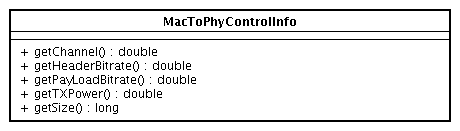
\includegraphics[width = \textwidth]{modelling/MacToPhyCtrlInfo_members.png}
 \caption{MacToPhyControlInfo interface}
 \label{fig: MacToPhyCtrlInfo interface}
\end{figure}

\h{\bp} is responsible for creating AirFrame and Signal and attaching
information (parameters) to them. For detailed arrangement of information in
Signal and AirFrame see \ref{AirFrame and Signal}.
When the AirFrame is complete and sent, \h{\bp} schedules a TX\_OVER message to
the \h{\bm} (via control-message).

\begin{figure}[H]
 \centering
 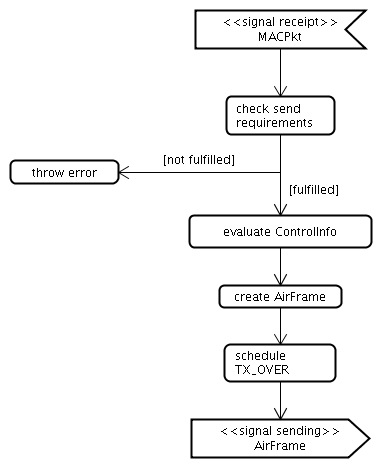
\includegraphics[width = 0.8\textwidth]{modelling/onMACPkt.png}
 \caption{sending process}
 \label{fig: sending process}
\end{figure}
\newpage



\subsection{Receiving and processing an AirFrame}

On arrival of an AirFrame \h{\bp}:
\begin{enumerate}
	
	% \item optional propagation delay, \h{\bp} updates the starting time of
%the Signal\req{rcvSimDelay},
	% \item reception of the preamble\req{rcvSimPreamble},
	\item applies AnalogueModels to the corresponding
Signal\req{rcvSimAttenuation},
	% \item decision whether packet is considered noise (Decider),
	\item receives the AirFrame\req{rcvSimDuration}.
\end{enumerate}

\begin{figure}[H]
 \centering
 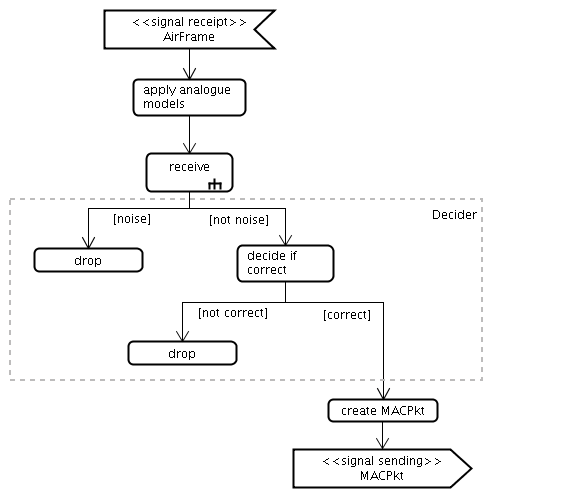
\includegraphics[width = 0.8\textwidth]{modelling/onAirFrame.png}
 \caption{receiving process}
 \label{fig: receiving process}
\end{figure}


The receiving process works as follows: In general time intervals during
reception are simulated by scheduling the AirFrame accordingly.
An optional propagation delay is simulated by updating the starting time of the
Signal\req{rcvSimDelay} according to the delay and scheduling the AirFrame to
the reception start point (\textit{stage 0}).\\

On reception start the Decider is asked for the time point\reqdef{decider} the
decision whether the signal is considered \textit{signal} or \textit{noise} is
made. The AirFrame is scheduled to that time point (\textit{stage 1}).\\

Next the Decider makes the decision (\textit{signal} / \textit{noise}) and the
AirFrame is scheduled to the time point when the receiving process is over
(\textit{stage 2}).\\

Finally reception is over and the AirFrame is completely received in reality
(\textit{stage 3}).

\begin{figure}[H]
 \centering
 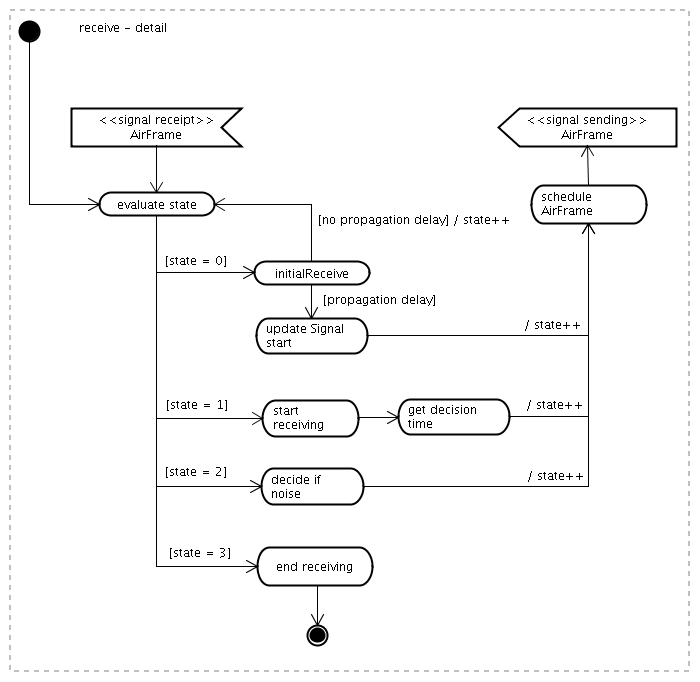
\includegraphics[width = \textwidth]{modelling/receive_detail.png}
 \caption{receive detail}
 \label{fig: receive detail}
\end{figure}

Right now the AirFrame is either dropped (if considered \textit{noise}) or
processed.

If processed, the corresponding SNInfo is given to the Decider to obtain a
DecisionResult that contains at least whether the AirFrame was received
correctly or not.

If not it is dropped now, otherwise \h{\bp} creates an appropriate MacPkt and
sends it up to MAC layer. Nevertheless we can also pass any signal received up
to MAC layer.

\textbf{Please note:} 'dropped' in this context means that \h{\bp} doesn't want
to treat the signal as \textit{signal}.


% The receiving process is modelled internally by a state machine that schedules
%the AirFrame that is received (since we have a pointer to it from the
%beginning) everytime a delay/time interval shall be simulated. That saves us
%the creation of additional self-messages.




%When the preamble of a packet is completely received, \h{\bp} constructs a
%SNInfo for the preamble, applies the AnalogueModels to it and passes it to the
%Decider to find out whether this packet is considered noise.

%\begin{figure}[H]
% \centering
% 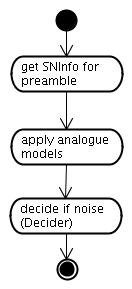
\includegraphics[width = 0.2\textwidth]{modelling/end_preamble_detail.png}
% \caption{end preamble detail}
% \label{fig: end preamble detail}
%\end{figure}

%In case a received packet is not \textit{noise} it is processed, i.e. \h{\bp}
%creates the corresponding SNInfo for the packet, applies AnalogueModels to it
%and passes the result to the Decider to check whether the packet was received
%correctly. If so, a MacPkt is created and handed up to
%Phy-Layer\req{rcvPassToMAC}.


\subsection{the .ned-file}

The .ned-file of the \h{\bp} has the following parameters:

\begin{itemize}
\item usePropagationDelay as \textit{boolean}\req{confDelay}
\item analogueModels as \textit{XML}\req{confAnalogue}\req{confAnalogueParam}
\item decider as \textit{XML}\req{confDecider}\req{confDeciderParam}
\item thermalNoise as \textit{numeric const}\req{confNoise}
\item sensitivity as \textit{numeric const}\req{confSens}
\item maximal TX power as \textit{numeric const}\req{confMaxTXPower}
\item switchTimeRX as \textit{numeric const}\req{confSwitchingTimes}
\item switchTimeTX as \textit{numeric const}\req{confSwitchingTimes}
\item switchTimeSleep as as \textit{numeric const}\req{confSwitchingTimes}
\end{itemize}

The parameters "analogueModels" and "decider" holds which AnalogueModels and
Decider to be used together with their parameters in XML format. The exact
format still has to be declared!

%\subsection{provide status information to MAC}

%Passively provided information\req{provpassive}: \h{\bm} is equipped with a
%reference to \h{\bp} in order to obtain information
%about channelstate\req{channelstate} and current radio state\req{currentmode}
%by
%simple method calls. \\
%Actively provided information\req{provactive}: A cMessage of the kind TX\_OVER
%is sent to MAC layer when a sending transmission is over\req{txover},
%\saf{sending process}.



%\subsection{send packets}

%Since \h{\bm} has a reference to \h{\bp} it can obtain information about the
%state the radio is is currently in\req{sendPreqMode}, it is not already sending
%to the channel on its own\req{sendPreqSending} and the channel is
%idle\req{sendPreqIdle} via method calls, \saf{BasePhyLayer interface}.

%The class MacToPhyControlInfo is designed as the container for control
%info\req{packetFromMac} the MAC layer
%wants to attach to the packet given down to Phy-Layer for sending.
%The packet itself is handed down as a MacPkt via OMNeT-channel. 